\documentclass[fleqn]{LxSymp_2026_Paper_Format}
\usepackage[T1]{fontenc}
\usepackage{mathpazo}
\usepackage{lmodern}
\usepackage{textcomp}
% add dot to section numbering
% add natbib and use apa style

\begin{document}

\title{Title of the Full Paper for the LISBON Laser Symposium 2026}
%\paperdoi{}
\firstpagehead{}
\runningheads{22nd LISBON Laser Symposium 2026}{}
\runnigfoots{}



\author{A. Abcde$^{\text{1},*}$, C. Fghij$^{\text{2}}$, K. Mnopqr$^{\text{3}}$}

\address{1: Dept. of Xxxxxxx Eeeeee, The University of Tabcd, Country\\
2: Dept. of Yyyyyyy Fffffff, The University of Wabcd, Country\\
3: Dept. of Zzzzzzz Ggggggg, The University of Yabcd, Country\\
\vskip 1pt
{\addressize{*Corresponding author:
\href{mailto:email@adress.xxx.yz}{\textstyleInternetlink{email@adress.xxx.yz}}}}}
\fontfamily{phv}\fontseries{mc}\fontsize{9}{10}\selectfont
\linespread{1.2}
\vskip 3 mm
\begin{center}
    \textbf{Keywords: }PIV processing, Micro PIV, Microfluidics, Heat transfer.
\end{center}
\vskip 8 mm
\abstract{\noindent
Please write your abstract here in 10 pt. font with approximately 300-400 words. Please write your abstract here in 10 pt. font with approximately 300-400 words. Please write your abstract here in 10 pt. font with approximately 300-400 words. Please write your abstract here in 10 pt. font with approximately 300-400 words. Please write your abstract here in 10 pt. font with approximately 300-400 words. Please write your abstract here in 10 pt. font with approximately 300-400 words. Please write your abstract here in 10 pt. font with approximately 300-400 words. Please write your abstract here in 10 pt. font with approximately 300-400 words. Please write your abstract here in 10 pt. font with approximately 300-400 words. Please write your abstract here in 10 pt. font with approximately 300-400 words. 
}

\section{Introduction}
\label{Sec:Intro}

This is the template to prepare the full paper manuscript for the 22$^\textrm{nd}$ International Symposium on Applications of Laser and Imaging  Techniques to Fluid Mechanics. Please follow the guidelines below:

\begin{itemize}
    \item Page size format is a 4:3 Aspect Ratio ($280~mm~\times~210~mm$). \textbf{There is no limit for the total number of pages.}
    \item Do not abbreviate the first and last names. Only middle names can be written with initials. 
    \item Use the template supplied and do not make your own \LaTeX File in any other format.
    \item In Equations, use the appropriate \LaTeX environment. Here is an example:
\end{itemize}
\begin{ceqn}
\begin{align}
    r_k\frac{DV_k}{Dt} = -\Tilde{N}P_k+\Tilde{N}\times t_k+r_k g
    \label{Eq:Example1}
\end{align}
\end{ceqn}
We recommend the use of labels for all sections, subsections, equations, figures, tables, etc., for easy reference. For example, as in Eq.~(\ref{Eq:Example1}) or Fig.~\ref{fig:drawing}. We recommend that you add new equations, figures, or tables by copy-pasting the previous code, and do not forget to change the labels.

\begin{figure}[htbp]
    \centering
    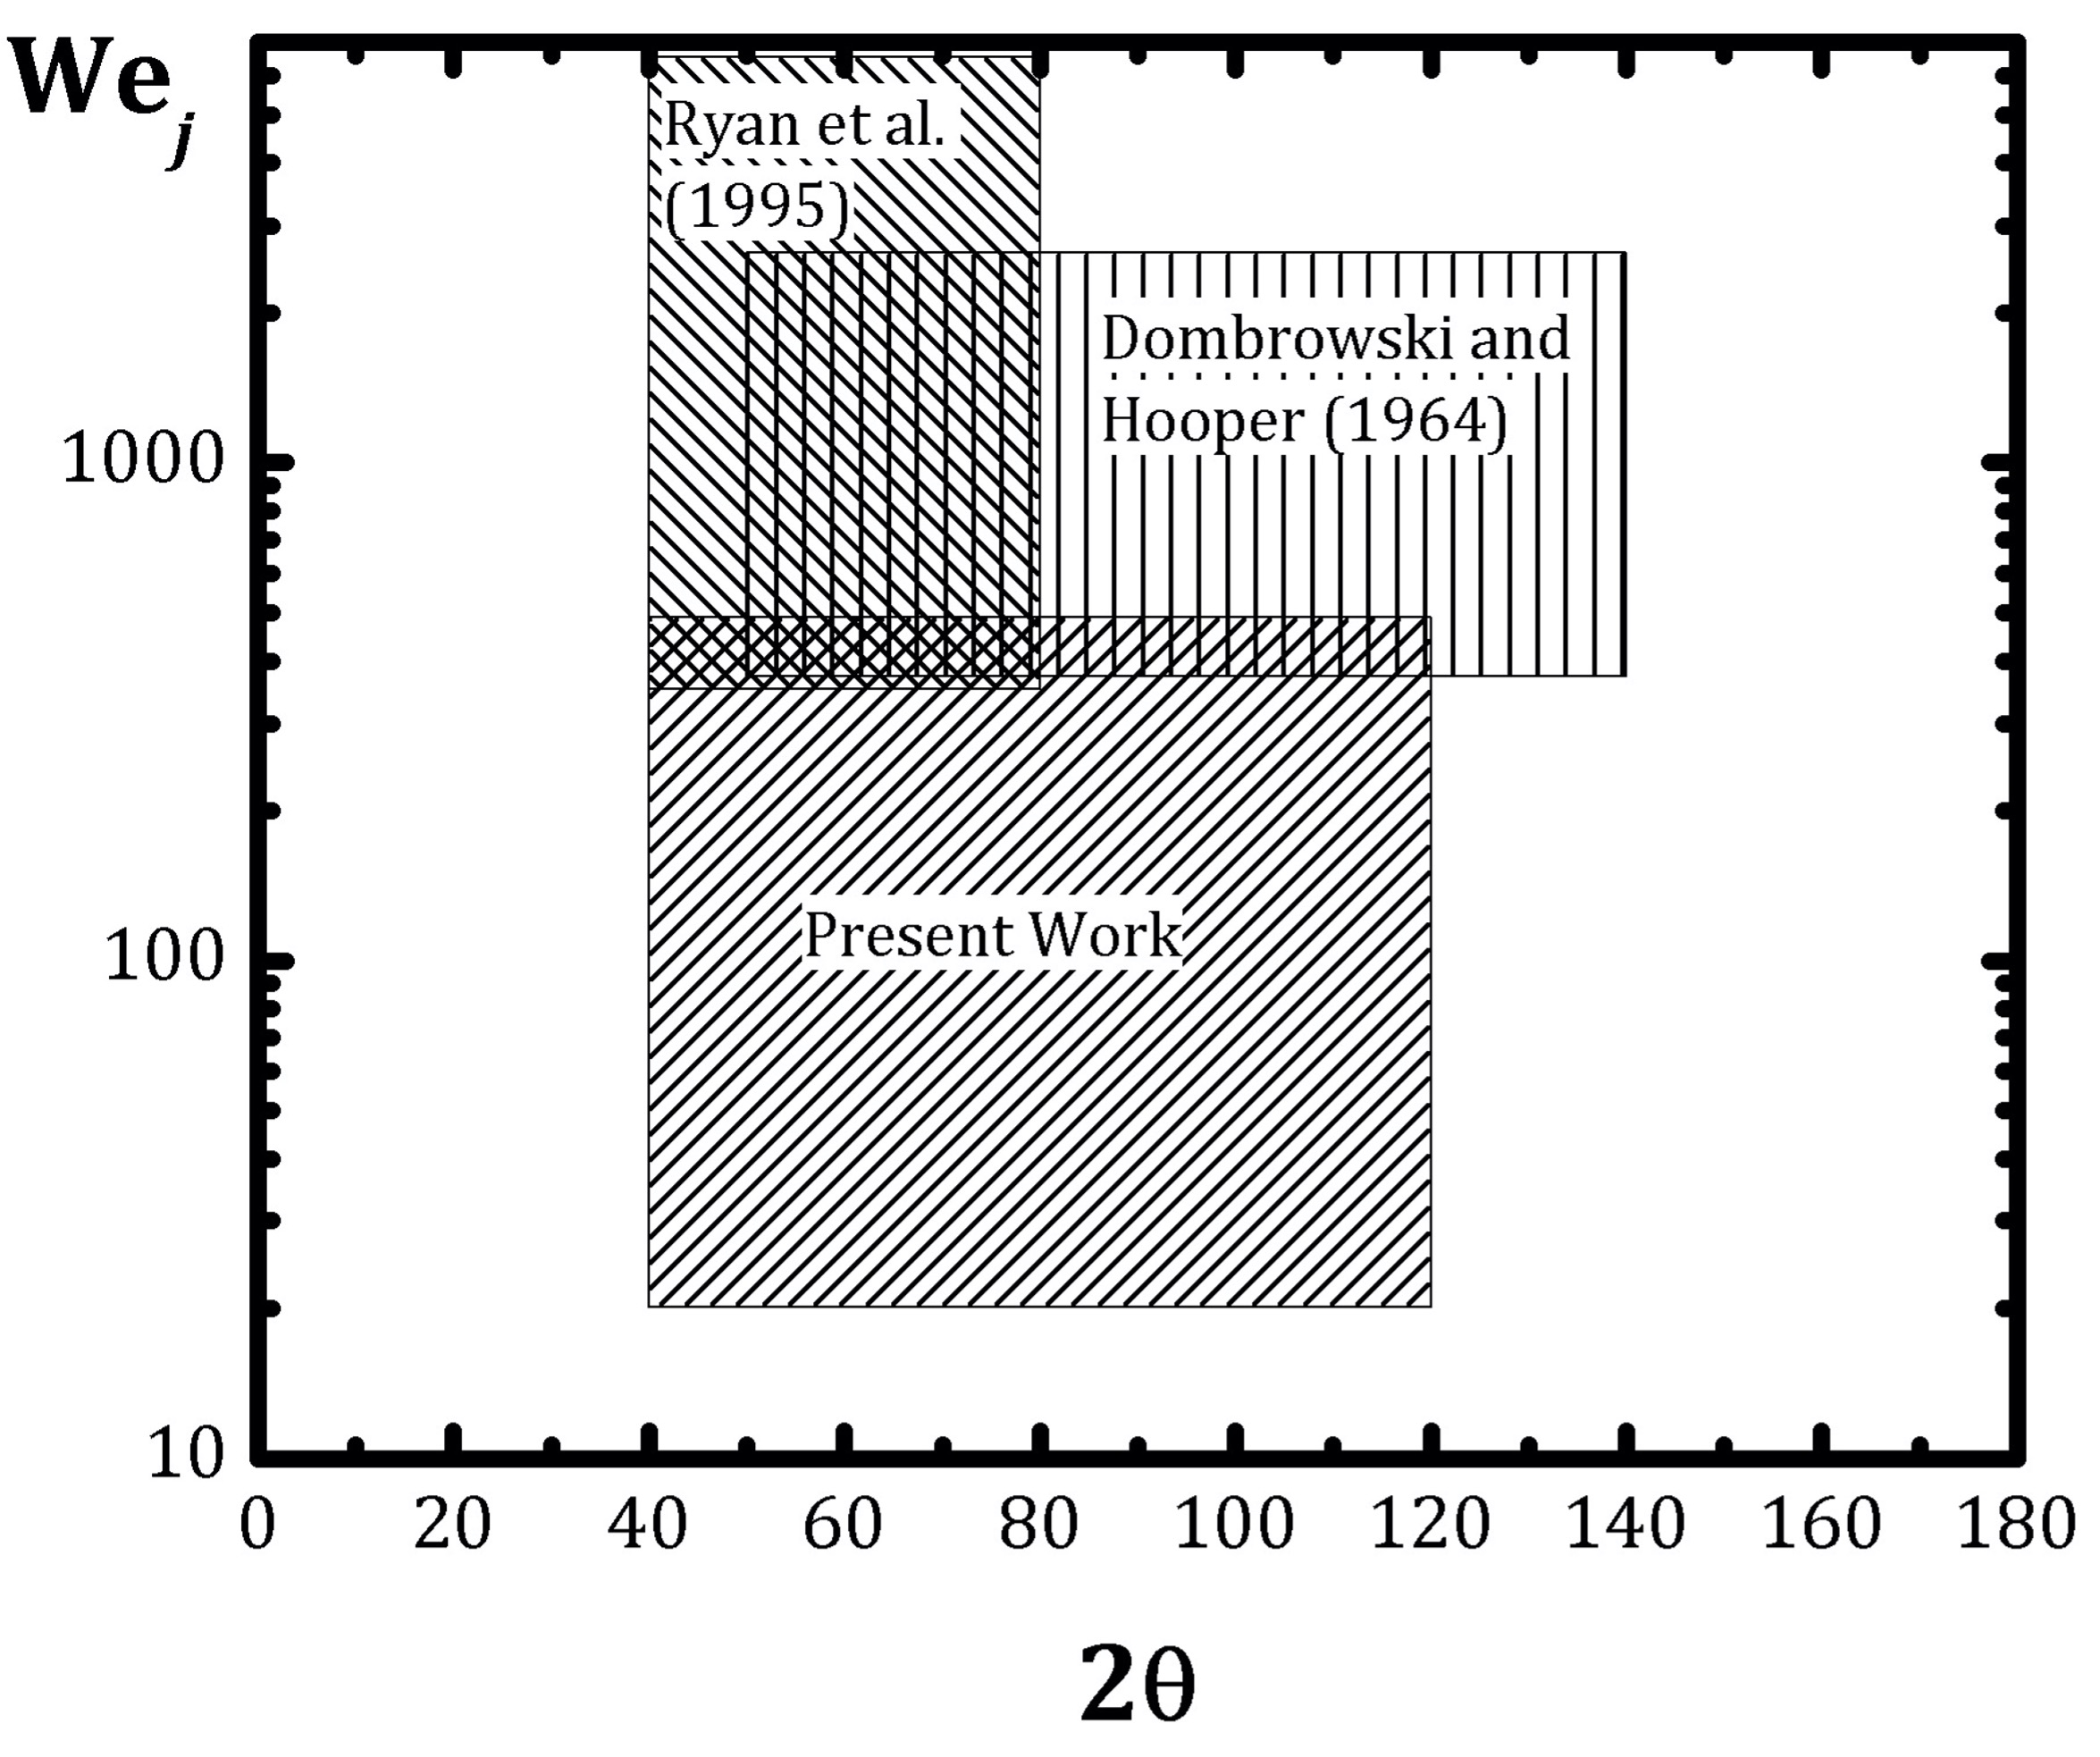
\includegraphics[width=0.5\textwidth]{Picture 1.jpg}
       \centering
    \caption{Example of a figure. Caption in Arial, font size 8, centered, Figure and figure number bold. Spacing before caption is 6 pt.}
    \label{fig:drawing}
\end{figure}

If you need to force the positioning of a figure, use [H] instead of [htbp].

\textbf{This is a manuscript version for \LaTeX.}

\section{Submission of the paper manuscript}
\label{Sec:Submission}

Upload the abstract up to \textbf{June 1st, 2026} at the site through your account following two simple steps.

\textbf{\# 1.} Access the ``My Congress'' area, which opens after acceptance.

\begin{figure}[H]
    \centering
    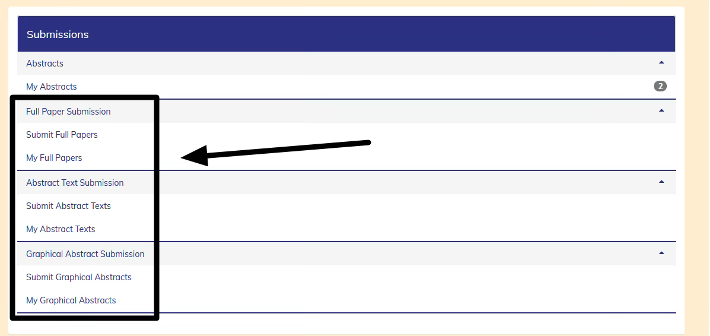
\includegraphics[width=0.5\textwidth]{Picture 2.png}
       \centering
    \caption{Step 1. Access the “My Congress” area which opens after acceptance.}
    \label{fig:drawing2}
\end{figure}

\textbf{\# 2.} Upload the “Full Manuscript” and the information for the “Abstract Text Submission” and “Graphical Abstract” in their corresponding fields, later used in the Symposium App.

\begin{figure}[H]
    \centering
    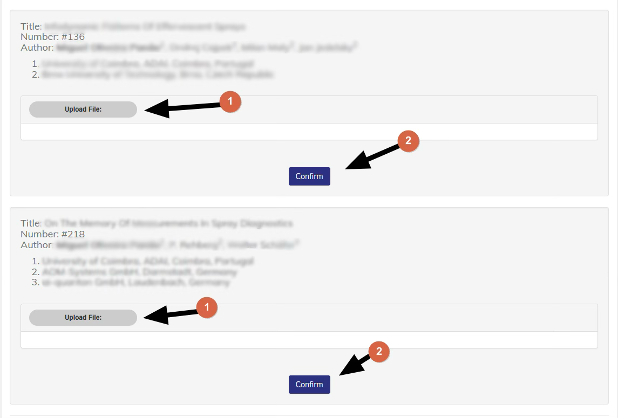
\includegraphics[width=0.5\textwidth]{Picture 3.png}
       \centering
    \caption{Step 2. Upload the “Full Manuscript” in the corresponding fields.}
    \label{fig:drawing3}
\end{figure}

\textit{Please avoid sending the paper by e-mail} and do it only if absolutely necessary. If you have any questions, send an e-mail to \href{mailto:publications@lisbon-lasersymposium.org}{publications@lisbon-lasersymposium.org}. 

\section{Permissions}
\label{Sec:permissions}

You are responsible for ensuring that you have the right to publish everything in your paper. If you use material from a copyrighted source, you may need to obtain permission from the copyright holder. You need to seek permission to use a figure or table if it has not been changed in any substantive way from the original or if it does not plot or compile data that are readily available to anyone. You need to seek permission to quote material if you use it in a way that is competitive with the original material, that is, if your use of the material will harm the rights of the original publisher and/or author. This criterion holds true regardless of the length of the quote. If the quoted material is not used competitively, you need only to cite the original source. Please consult your own legal adviser if you have any questions about what may require permission.

%\clearpage

\begin{table}[htp]
\centering\label{tab:template}
\caption{Example of a table. Caption in Palatino, font size 10, centered, Table, and table number bold.}
\vspace{6pt}
\begin{tabular}{c|ccc}
\toprule
  & Column 1 & Column 2 & Column 3 \\
\midrule 
Row 1 & 5 & 34 & 67\\
Row 2 & 6 & 45 & 75\\
Row 3 & 7 & 46 & 64\\
Row 4 & 8 & 56 & 53\\
%\bottomrule 
\end{tabular}
\end{table}

Please use SI units in all texts, figures, and tables.

\section{Conclusions}
\label{Sec:Conclusions}

For further assistance, please refer to the LISBON Laser Symposium 2024 website or contact our staff at \href{mailto:helpdesk@lisbon-lasersymposium.org}{helpdesk@lisbon-lasersymposium.org}.

\section*{Acknowledgements}
The authors would like to acknowledge...
%\bigskip

\section*{Nomenclature}
\begin{tabbing}
\hspace*{1.18 cm}  \= \hspace*{4 cm}  \kill
$a$ 	\>	Acceleration [m s$^2$]    \\
$F$		\> 	Force [N]	\\
$m$ 	\> 	Mass [kg]
\end{tabbing}
%\bigskip

References use the APA format. You can use Google Scholar to search for the reference, select ``Cite'' and there is a BibTeX option that you can copy and paste directly into your bib file. You can cite works from a journal \citep{foucaut2004piv}, book~\citep{yarin2017collision}, or book chapter~\citep{armstrong1988laser} with \verb|\citep{}| to include the reference next to the text or \verb|\citet{}| to add the reference as part of the text, for example, `...according to~\citet{panao2018spray}''.


\bibliography{LxSymp2026_Bib}
\bibliographystyle{apacite}

% \vspace{0.5cm}
% \begin{thebibliography}{99}
% \bibitem{ref:Payri}Payri, R., Gimeno, J., Marti-Aldaravi, P., Vaquerizo, D., 2016, \textit{Atomization and Sprays}, 26 (9), pp. 889-919.
% \bibitem{ref:Wilcox}Wilcox, D.~C., 1993, ``Turbulence Modelling for CFD''. DCW Industries, Inc.
% \bibitem{ref:Lampa}Lampa, A., and Fritsching, U., Sep. 5.-7. 2011, 24th European Conference on Liquid Atomization and Spray Systems.
% \bibitem{ref:ilass} Institute for liquid atomization and spray systems, {\ULurl{http://ilasseurope.org/events/ilass-europe-2020/}}
% \end{thebibliography}



\end{document}
